\documentclass[10pt]{beamer}

\usetheme[progressbar=frametitle, titleformat=smallcaps]{metropolis}
\usepackage{appendixnumberbeamer}

\usepackage{booktabs}
\usepackage[scale=2]{ccicons}

\usepackage{pgfplots}
\usepgfplotslibrary{dateplot}

\usepackage{xspace}
\newcommand{\themename}{\textbf{\textsc{metropolis}}\xspace}

\newcommand{\nuc}[2]{${}^{#1}\textrm{#2}$}
\newcommand{\mnuc}[2]{{}^{#1}\textrm{#2}}
\newcommand{\react}[4]{$#1(#2,#3)#4$}
\newcommand{\mreact}[4]{#1(#2,#3)#4}
\newcommand{\alpa}{\react{\mnuc{27}{Al}}{\textrm{p}}{\alpha}{\mnuc{24}{Mg}}}
\newcommand{\nag}{\react{\mnuc{14}{N}}{\alpha}{\gamma}{\mnuc{18}{F}}}
\newcommand{\squared}{${}^{2}$}

\title{
    Verification of Recoil Separator Properties Through Reaction Measurements
}
\subtitle{}
% \date{\today}
\date{November 9, 2018}
\author{Michael T Moran}
\institute{Doctoral Defense\\University of Notre Dame}
% \titlegraphic{\hfill\includegraphics[height=1.5cm]{logo.pdf}}

\begin{document}

\maketitle

% \begin{frame}[fragile]{Table of Contents}
%   \setbeamertemplate{section in toc}[sections numbered]
%   \tableofcontents[hideallsubsections]
% \end{frame}

\section{Introduction}

\begin{frame}[fragile]{Capture Reactions}

    Primary burning processes for energy production depend on the
    properties of the star

    Hydrogen burning:
    \begin{itemize}
        \item low mass: $pp$-chains
        \item massive stars: CNO, NeNa, and MgAl cycles
    \end{itemize}

    Helium burning:
    \begin{itemize}
        \item \react{\mnuc{4}{He}}{\alpha\alpha}{\gamma}{
            \mreact{\mnuc{12}{C}}{\alpha}{\gamma}{
            \mreact{\mnuc{16}{O}}{\alpha}{\gamma}{
            \mreact{\mnuc{20}{Ne}}{\alpha}{\gamma}{\mnuc{24}{Mg}}}}}
        % \item Triple-$\alpha$ process and \react{\mnuc{12}{C}}{\alpha}{\gamma}{\mnuc{16}{O}}
    \end{itemize}

    Additional He reactions:
    \begin{itemize}
        \item main sources of neutrons for $s$-process:
            \react{\mnuc{13}{C}}{\alpha}{\rm n}{\mnuc{16}{O}} and
            \react{\mnuc{22}{Ne}}{\alpha}{\rm n}{\mnuc{25}{Mg}} (AGB
            stars)
        \item reactions on ashes of cyclic H burning (e.g.
            \react{\mnuc{14}{N}}{\alpha}{\gamma}{\mnuc{18}{F}})
    \end{itemize}

\end{frame}

\begin{frame}[fragile]{Radiative Capture}

    Reactions: $({\rm p}, \gamma)$ and $(\alpha,\gamma)$ (in general, \react{A}{a}{\gamma}{B})
    \begin{itemize}
        \item studied by detecting $\gamma$-ray produced
    \end{itemize}

    % Reactions like \react{A}{a}{\gamma}{B} (e.g. $({\rm p}, \gamma)$, $(\alpha,\gamma)$)

    Detecting the $\gamma$ can be difficult due to:
    \begin{itemize}
        \item large background count rates (move underground)
        \item low count rates (measure only resonances)
        \item limited detector efficiency
    \end{itemize}

    % Studied focused primarily on resonances to reduce the effect of
    % these problems

\end{frame}

\begin{frame}[fragile]{Inverse Kinematics}

    Perform reaction in inverse kinematics: \react{a}{A}{B}{\gamma}

    \begin{itemize}
        \item heavy projectile impinges on light target (H or He)
        \item heavy recoil escapes the target
        \item detect with high-efficiency detector
    \end{itemize}

    Incident beam also passes through the light target, so we need to
    \textbf{stop the beam} from reaching our detector

\end{frame}

\section{Recoil Separation}

\begin{frame}[fragile]{St.\ George}

    % \vspace{1.5em}
    \begin{figure}
        \includegraphics[width=0.95\textwidth]%
            {figures/stg.png}
    \end{figure}

    \tiny{Couder \textit{et al.}, 2008}  % check if this looks OK

\end{frame}

\begin{frame}[fragile]{Particle Selection}

    Uniquely identify particles by charge, energy, mass, and momentum
    % \[
    %     \begin{split}
    %         B\rho = \frac{\sqrt{2mT}}{q} = \frac{p}{q}
    %     \end{split}
    %     \quad\quad\quad
    %     \begin{split}
    %         E\rho = \frac{2T}{q}
    %     \end{split}
    % \]

    \begin{alertblock}{Magnetic Selection}<2->
        \[
            B\rho = \frac{\sqrt{2mT}}{q} = \frac{p}{q}
        \]
    \end{alertblock}
    \begin{alertblock}{Electric Selection}<3->
        \[
            E\rho = \frac{2T}{q}
        \]
    \end{alertblock}
    \begin{alertblock}{Wien Filter Selection}<4->
        \[
            v = \frac{E\rho}{B\rho}
        \]
    \end{alertblock}

    % $B\rho$ and $E\rho$ are the magnetic and electric rigidities of the
    % particle in question

\end{frame}

\begin{frame}[fragile]{Angular and Energy Acceptance}

    Recoils leave target with a range of momentum/energy values and angles due to kinematics of the reaction
    \[
        \begin{split}
            p_{\rm recoil} = \sqrt{2m_AE_A} \pm p_{\gamma}
        \end{split}
        \quad\quad\quad
        \begin{split}
            \theta_{\rm recoil, max} = \arctan\left(\frac{p_{\gamma}}{\sqrt{2m_AE_A}}\right)
        \end{split}
    \]

    Recoils must be transported within defined parameter bounds
    \[
        \begin{split}
            \Delta E/E = \pm7.5\,\%
        \end{split}
        \quad\quad\quad
        \begin{split}
            \Delta\theta = \pm40\,\text{mrad}
        \end{split}
    \]

    These bounds must hold for all possible $E\rho$ and $B\rho$

\end{frame}

\begin{frame}[fragile]{Importance of Acceptances}

    In an experiment, all produced recoils must be transported to the detector plane

    Verifying the acceptance will:
    \begin{itemize}
        \item eliminate St.\ George as a potential source of uncertainty
        \item show the beam rejection properties are sufficient to measure the cross section
    \end{itemize}

    % Ensures that all of the produced recoils and none of the incident
    % beam particles for a given reaction reach the detector plane
    % \begin{itemize}
    %     \item produced recoils can be extremely rare (1 for every
    %         $10^{15}$ beam particles)
    % \end{itemize}

    Once verified for enough $B\rho$ and $E\rho$
    possibilities, separator has a \textbf{single tune} that is scaled to new values

\end{frame}

\section{Acceptance Measurements}

\begin{frame}[fragile]{Types of Acceptances}

    The goal is for 100\,\% of the particles to make it to the
    final detector plane
    \begin{itemize}
        \item ``particles'' are produced recoils or incident test beam
        \item measure with Faraday cups or particle detectors
    \end{itemize}

    % Can divide measurements between three possible cases:

    \begin{alertblock}{Energy}<2->%<1-| alert@4> for highlighting
        change the particle energy without interfering with other
        properties
    \end{alertblock}
    \begin{alertblock}{Angular}<3->
        change the deflection of the particle at the target location
    \end{alertblock}
    \begin{alertblock}{Joint}<4->
        adjust both at the same time
    \end{alertblock}

\end{frame}

\begin{frame}[fragile]{Energy Acceptance}

    For a particle beam with a given $B\rho$ and $E\rho$:

    \begin{itemize}
        \item Tune the test beam to a given energy, and
            tune St.\ George for that energy
        \item Verify 100\,\% transmission, adjust the tune
            if necessary
        \item Adjust the beam energy within the energy
            acceptance bounds and measure transmission
        \item Adjust the tune if necessary to have 100\,\%
            transmission for all possible energy changes within the
            acceptance bounds
    \end{itemize}

\end{frame}

\begin{frame}[fragile]{Energy Acceptance}

    \vspace{0.5em}
    Energy acceptance results in a single tune for St.\ George

    \begin{figure}
        \includegraphics[width=0.75\textwidth]%
            {figures/rigidity_phase_space.png}
    \end{figure}

    \tiny{Adapted from Meisel, \textbf{Moran}, \textit{et al.}, 2017}

\end{frame}

\begin{frame}[fragile]{Angular Acceptance}

    For a particle beam with a given $B\rho$ and $E\rho$:

    \begin{itemize}
        \item Tune the test beam to a given energy, and
            tune St.\ George for that energy
        \item Verify 100\,\% transmission, adjust the tune
            if necessary
        \item ``Deflect'' the beam at the target location
            within the acceptance bounds (horizontally and vertically)
        \item Adjust the tune if necessary to have 100\,\%
            transmission for all possible angular changes within the
            acceptance bounds
    \end{itemize}

\end{frame}

\begin{frame}[fragile]{Joint Acceptance}

    All experiments will have an angular and energy spread, so must
    confirm that the acceptances can be achieved at the same time
    % \begin{itemize}
    %     \item Following the previous procedures, but interwoven, would
    %         take too long for each point
    % \end{itemize}

    Can use a degrader foil to create an angular and energy spread at the same time
    \begin{itemize}
        \item target properties matched to test beam selection
        \item limited by diagnostic equipment (can't use a detector due to high-intensity beam)
        \item energy and angular distribution make it more difficult to refine the tune if we don't have 100\,\% transmission
    \end{itemize}

\end{frame}

\section{Reaction Measurements}

\begin{frame}[fragile]{Justification for Reaction Measurements}

    Use the known kinematics of the reaction to gradual move toward a full acceptance solution
    \begin{itemize}
        \item known cross section, angular and energy distribution, etc.
        \item tune so that 100\,\% of the produced particles captured by detector (can check with incident beam as well)
        \item St.\ George then has \textit{at least} the acceptance necessary for the reaction
    \end{itemize}

\end{frame}

\begin{frame}[fragile]{The \alpa{} Reaction}

    Focus on two isolated resonances:
    \begin{itemize}
        \item high energy: $E_{\rm p} = 1.36$~MeV \textrightarrow{} $E_{\alpha} = 2.77$~MeV
        \item low energy: $E_{\rm p} = 1.18$~MeV \textrightarrow{} $E_{\alpha} = 2.59$~MeV
        \item both are $2+$ resonances with isotropic angular distribution
    \end{itemize}

    For both reactions, kinematics and target effects give $\Delta E/E = \pm 3$\,\%

\end{frame}

\begin{frame}[fragile]{The \alpa{} Reaction}

    \vspace{0.5em}
    Cross section is well-known, reducing it as an uncertainty in the
    measurements

    \begin{figure}
        \includegraphics[width=0.75\textwidth]%
            {figures/zero_degree_pa0.png}
    \end{figure}

    \tiny{Courtesy of R.\ J.\ deBoer, 2017}

\end{frame}

\begin{frame}[fragile]{Angular Acceptance Measurement}

    The reaction \alpa{} emits the $\alpha$ particles within an
    isotropic angular distribution
    \begin{itemize}
        \item target cup aperture limits entrance to $\approx 40$~mrad acceptance
        \item we will attempt to transport all $\alpha$ particles (based on the cross section) to the detector
    \end{itemize}

\end{frame}

\begin{frame}[fragile]{Alternate Tune}

    Due to limits of previous work at the time, we have to move our detector system up to the Wien filter focal plane
    \begin{itemize}
        \item can replicate this work once angular acceptance measurements extended to last section of St.\ George
        \item beam suppression is sufficient to reject the incident proton beam before the detector
        \item ``canonical'' St.\ George tune cannot be used
    \end{itemize}

    This is an alternate to a full acceptance measurement with St.\ George (limited energy acceptance, subset of separator)
    \begin{itemize}
        \item built upon previous acceptance measurements
        \item direct He beam used to verify acceptance before experiment at resonance energies
    \end{itemize}

\end{frame}

\begin{frame}[fragile]{Alternate Tune}

    \vspace{1em}
    Determined expected field strengths using \verb+COSY+ and verified
    with direct particle transport before the experiment

    \begin{figure}
        \includegraphics[width=0.75\textwidth]%
            {figures/optimal_tune_x.png}<1>
        \includegraphics[width=0.75\textwidth]%
            {figures/optimal_tune_y.png}<2>
    \end{figure}

\end{frame}

% include equation for acceptance, maybe new slide?
% say how you verified on-resonance with direct He beam

\begin{frame}[fragile]{Acceptance}

    We can relate the yield at our detector to what we expect from the cross section to determine our angular acceptance

    \[
        \theta = \arccos\left(1 - 2\frac{Y_{\rm experiment}}{Y_{\rm theory}}\right)
    \]

    This assumes a ``symmetric'' acceptance (constant opening angle for acceptance cone)
\end{frame}

\begin{frame}[fragile]{Acceptance Measurements}

    % \vspace{0.5em}
    \begin{figure}
        \includegraphics[width=0.85\textwidth]%
            {figures/acceptance_uncertainty.png}
    \end{figure}

\end{frame}

\begin{frame}[fragile]{Acceptance Uncertainty}

    We can attribute the uncertainty at each measurement to the
    underlying variables within our control: energy, current, time, and
    target thickness
    \begin{itemize}
        \item $E_{\rm res}$ and higher: dominated by current uncertainty
        \item energies lower than $E_{\rm res}$: dominated by energy uncertainty
        \item final irreducible uncertainty (cross section, counting statistics, etc.) cannot be avoided
        % \item attribution through a hybrid Monte Carlo/Bayesian approach
    \end{itemize}

    Attribution is done through a hybrid Monte Carlo/Bayesian approach, where we adjust our priors and observe the change in the outcome

    % Final irreducible uncertainty cannot be avoided, but controllable
    % uncertainty can be minimized

\end{frame}

\begin{frame}[fragile]{Uncertainty Decomposition}

    \vspace{1em}
    \begin{figure}
        \includegraphics[width=0.65\textwidth]%
            {figures/inputs.png}
    \end{figure}

\end{frame}

\section{Future Directions}

\begin{frame}[fragile]{Experimental Outcome}

    St.\ George has been shown to have the following acceptances:
    \begin{itemize}
        \item $\Delta E/E \geq \pm 7.5$\,\% and $\Delta\theta = 0$~mrad
        \item $\Delta E/E = \pm 3$\,\% and $\Delta\theta = \pm 40$~mrad
            (to WF)
    \end{itemize}

    Preliminary beam reduction measurements on the order of $10^{12}$

    Separation properties and beam currents are suitable for low-energy
    and off-resonance cross section measurements

\end{frame}

\begin{frame}[fragile]{The Future of St.\ George}

    \begin{itemize}
        \item St.\ George can be used for a restricted subset of
            experiments
        \item Ability to fine-tune the separator and verify its
            properties over a range of $B\rho$ and $E\rho$ values
            essential for future experiments
        \item Diagnostic equipment and procedures developed to be
            applied to future separators (SECAR)
        \item Final parts of the St.\ George system (HIPPO supersonic
            jet gas target, full detector system, additional
            diagnostics, etc) will unlock the full range of experimental
            work
    \end{itemize}

\end{frame}

\maketitle

\appendix

% potential slides:
% - tables showing the uncertainty values
% - detailed run plan
% - astrophysics support? PP, CNO, etc?
% - R-matrix (plus extra details)
% - STG planned reactions
% - detector spectra

\begin{frame}[fragile]{Hydrogen Burning}
    \begin{figure}
        \includegraphics[width=0.95\textwidth]%
            {figures/cno_nena_mgal.png}
    \end{figure}
\end{frame}

\begin{frame}[fragile]{Stellar Lifecyles}
    \begin{figure}
        \includegraphics[width=0.85\textwidth]%
            {figures/iliadis_lifecycle.png}
    \end{figure}

    \textbf{H}-C: Hydrogen burning in core; \textbf{He}-S: Helium
    burning in shell; \textbf{DU}: dredge up events

    \tiny{Iliadis, \textit{Nuclear Physics of Stars}, 2015}
\end{frame}

\begin{frame}[fragile]{Magnetic and Electric Rigidities}
    Elements within St.\ George are tuned for the $B\rho$ and $E\rho$ of
    the recoil particle
    \[
        \begin{split}
            B\rho = \frac{\sqrt{2mT}}{q}
        \end{split}
        \quad\quad
        \begin{split}
            E\rho = \frac{2T}{q}
        \end{split}
    \]

    Design limits: $0.1 \leq B\rho \leq 0.45$~Tm and $E\rho \leq 5.7$~MV
\end{frame}

\begin{frame}[fragile]{Particle Selection}
    \vspace{1em}
    Any two of the three possibilities may be combined to uniquely
    identify a particle

    \begin{figure}
        \includegraphics[width=0.75\textwidth]%
            {figures/particle_selection_by_field.png}
    \end{figure}
\end{frame}

\begin{frame}[fragile]{The \alpa{} Reaction}
    \vspace{1.5em}
    \begin{figure}
        \includegraphics[width=0.4\textwidth]%
            {figures/reaction_energy_diagram.png}
    \end{figure}
    
    For $\alpha_1$:
    \begin{itemize}
        \item \nuc{24}{Mg} first excited state: 1.368~MeV ($2+$)
        \item $E_{\alpha_1} \approx 1.8$~Mev (for higher resonance)
        % \item $E_{\gamma} = 1.368$~MeV
    \end{itemize}
\end{frame}

\begin{frame}[fragile]{95\,\% Contributions}
    \begin{figure}
        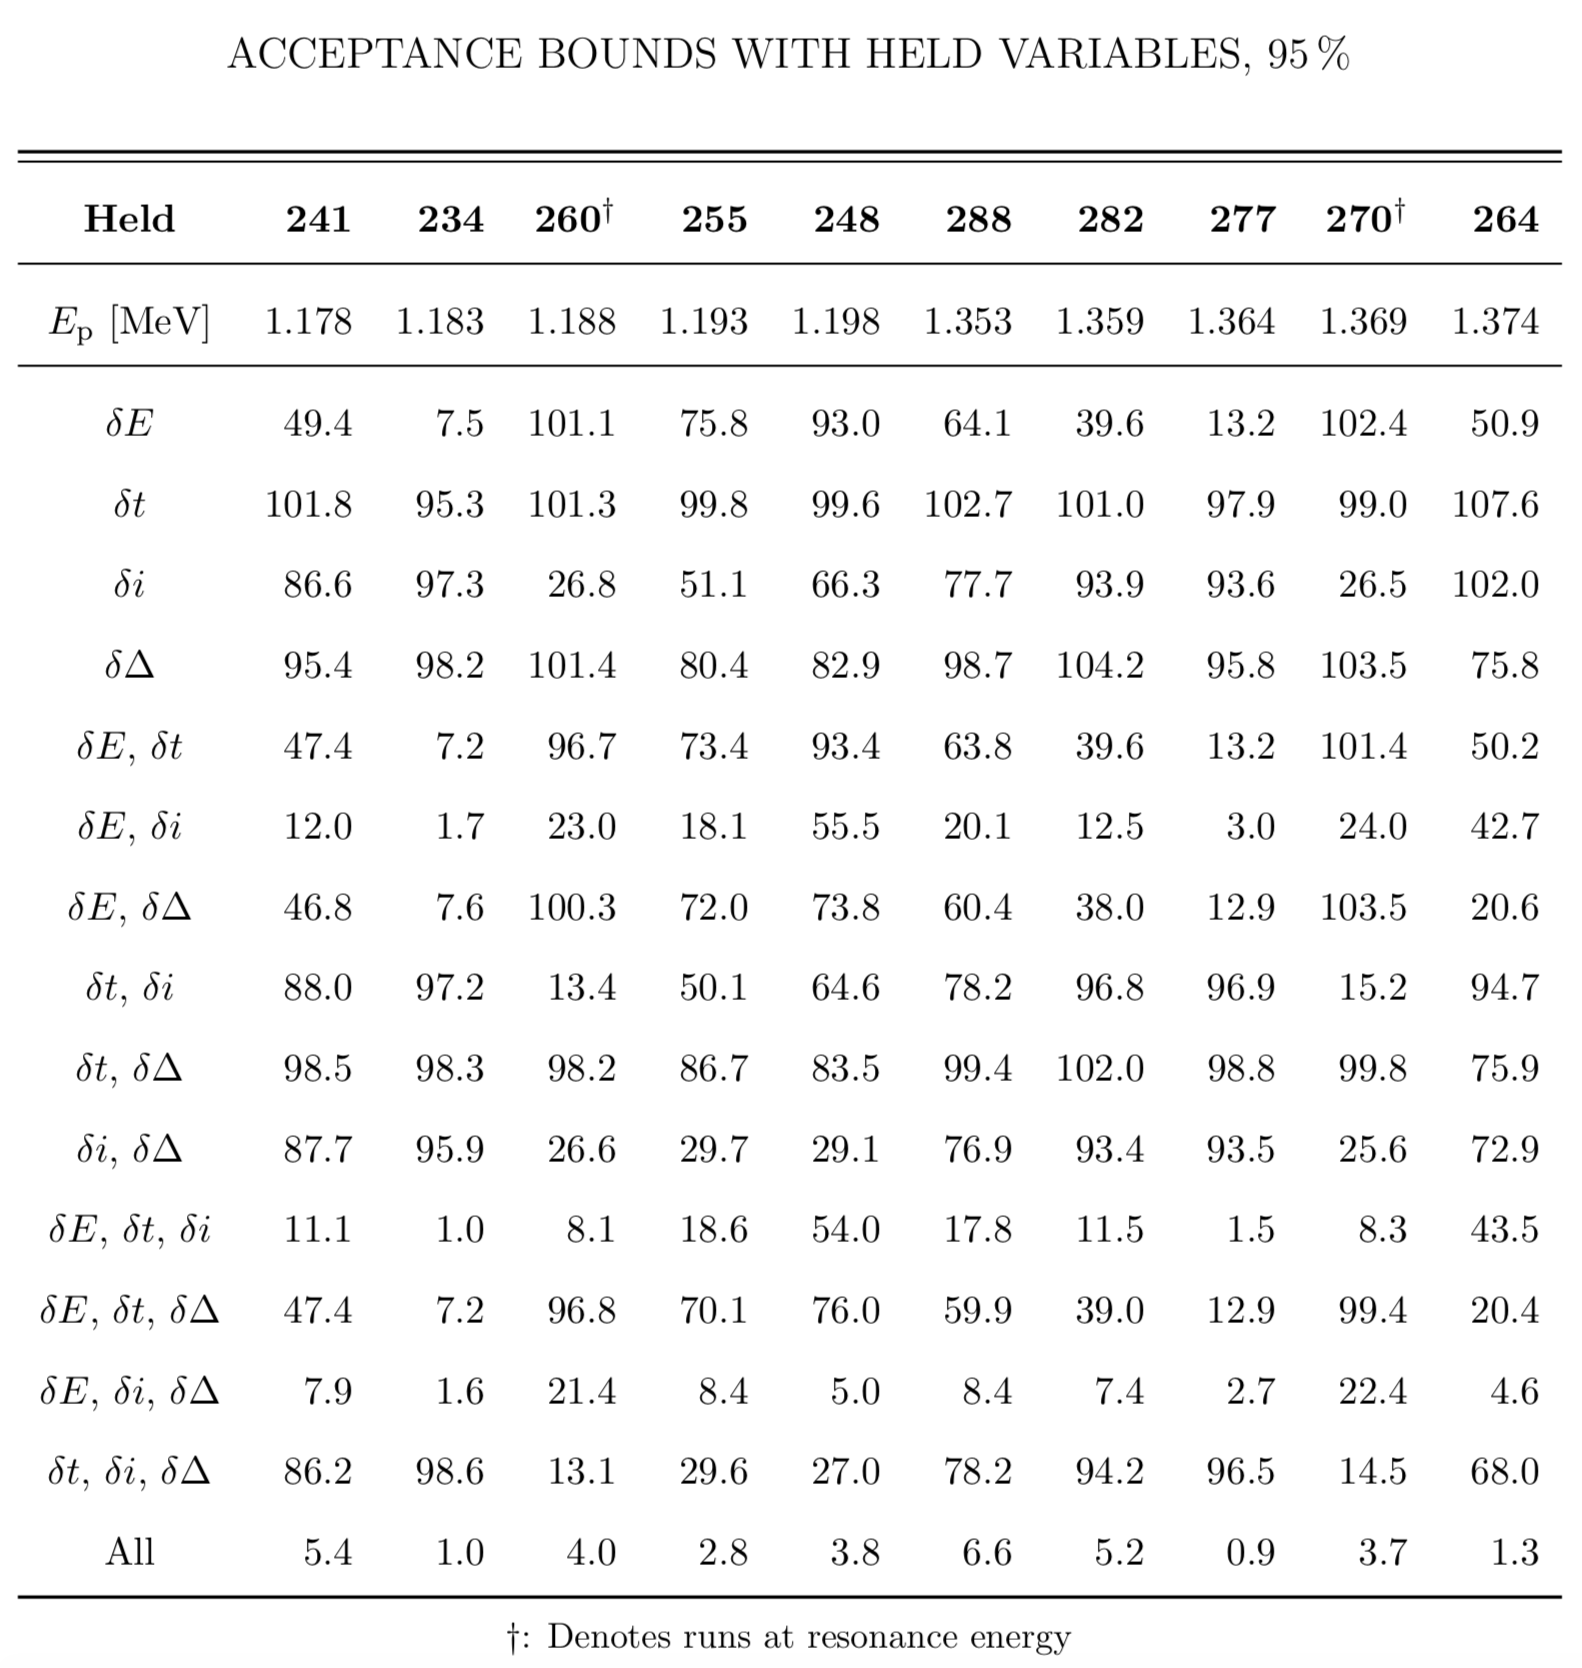
\includegraphics[width=0.7\textwidth]{figures/table_95.png}
    \end{figure}
\end{frame}

\begin{frame}[fragile]{Detector Spectrum}
    \vspace{0.5em}
    \begin{figure}
        \includegraphics[width=0.6\textwidth]%
            {figures/high_resonance_detector_strips.png}
    \end{figure}
\end{frame}

\begin{frame}[fragile]{Initial Test Reactions}
    \begin{figure}
        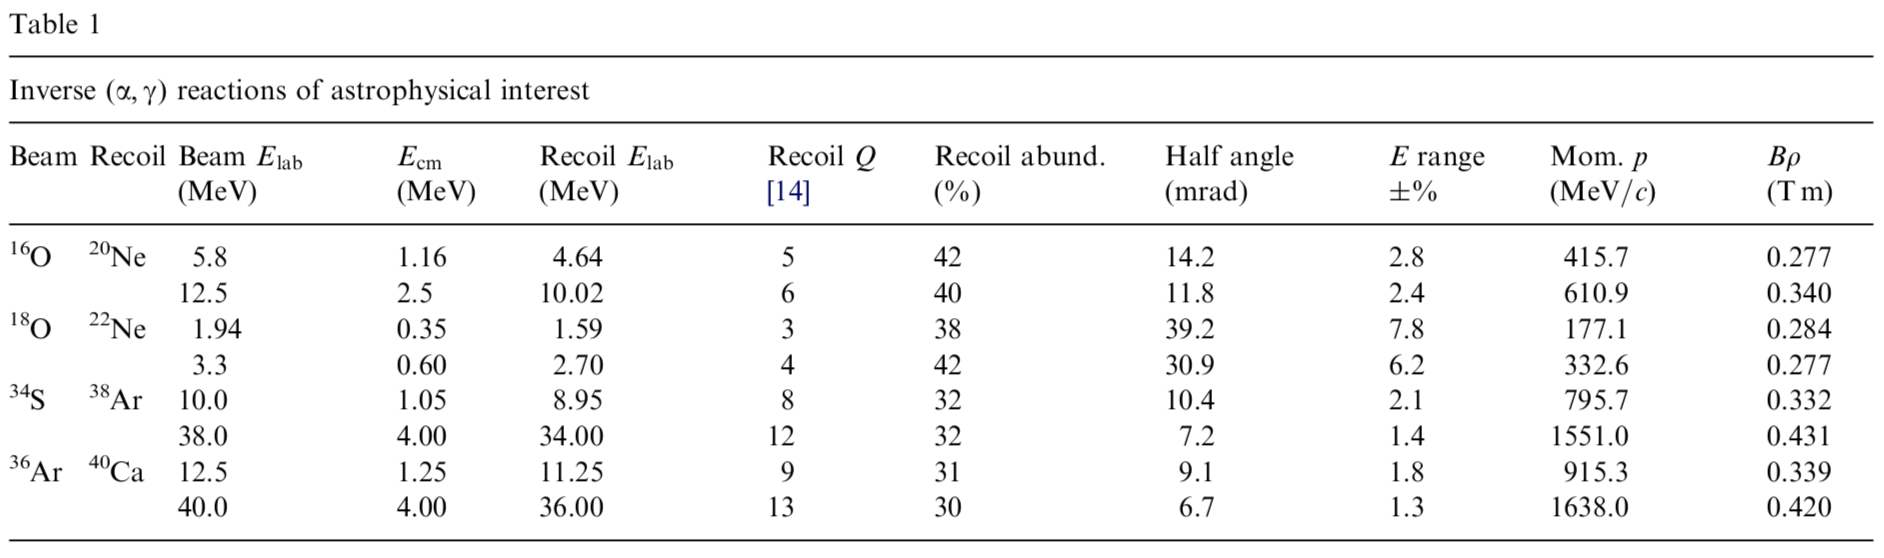
\includegraphics[width=\textwidth]{figures/stg_reactions.png}
    \end{figure}
\end{frame}

% \begin{frame}[allowframebreaks]{References}
%   \bibliography{defense}
%   \bibliographystyle{abbrv}
% \end{frame}

\end{document}
